\documentclass[11pt,a4paper]{article}

% --- Language & Encoding ---
\usepackage[utf8]{inputenc}
\usepackage[T1]{fontenc}
\usepackage{lmodern}

% --- Math and Physics ---
\usepackage{amsmath}
\usepackage{amssymb}
\usepackage{bm}

% --- Page Geometry ---
\usepackage[margin=1in, headheight=14.5pt]{geometry}

% --- Graphics & Tables ---
\usepackage{graphicx}
\usepackage{grffile}
\usepackage{booktabs}
\usepackage{array}

% --- Colors & Visual Styling ---
\usepackage{xcolor}
\definecolor{PrimaryColor}{HTML}{1A365D}   % Deep Navy Blue
\definecolor{SecondaryColor}{HTML}{2B6CB0} % Slate Blue
\definecolor{AccentColor}{HTML}{D69E2E}    % Warm Gold/Amber
\definecolor{LightBg}{HTML}{F7FAFC}        % Off-white/Gray
\definecolor{BorderColor}{HTML}{E2E8F0}    % Soft border gray

% --- Section Headers Styling ---
\usepackage{titlesec}
\titleformat{\section}
  {\normalfont\Large\bfseries\color{PrimaryColor}}{\thesection}{1em}{}[{\color{PrimaryColor}\titlerule[1.5pt]}]
\titleformat{\subsection}
  {\normalfont\large\bfseries\color{SecondaryColor}}{\thesubsection}{1em}{}
\titleformat{\subsubsection}
  {\normalfont\normalsize\bfseries\color{SecondaryColor}}{}{0em}{}

% --- Lists Customization ---
\usepackage{enumitem}
\setlist[itemize]{leftmargin=1.5em, itemsep=0.3em, topsep=0.3em}
\setlist[enumerate]{leftmargin=1.5em, itemsep=0.3em, topsep=0.3em}

% Custom checklists for Action Items
\newlist{todolist}{itemize}{2}
\setlist[todolist]{label=$\square$, leftmargin=1.5em, itemsep=0.3em, topsep=0.3em}
\newcommand{\doneitem}{\item[\rlap{\raisebox{0.15ex}{\hspace{0.1em}\checkmark}}$\square$]} % Custom checked box

% --- Headers & Footers ---
\usepackage{fancyhdr}
\pagestyle{fancy}
\fancyhf{}
\fancyhead[L]{\textcolor{SecondaryColor}{\bfseries Research Meetings with Shai}}
\fancyhead[R]{\textcolor{SecondaryColor}{\leftmark}}
\fancyfoot[C]{\thepage}
\renewcommand{\headrulewidth}{0.4pt}
\renewcommand{\footrulewidth}{0pt}

% --- Hyperlinks & Metadata ---
\usepackage[pdftex,
            pdfauthor={Yuval Kochavi},
            pdftitle={Research Meetings with Shai},
            pdfsubject={Marshak Wave & Radiation Transport Simulation Notes},
            colorlinks=true,
            linkcolor=SecondaryColor,
            urlcolor=SecondaryColor,
            citecolor=SecondaryColor]{hyperref}

% --- Custom Info Box for Meeting Details ---
\newcommand{\meetingmeta}[3]{
    \noindent
    \colorbox{LightBg}{
        \begin{minipage}{\dimexpr\textwidth-2\fboxsep\relax}
            \vspace{0.5em}
            \hspace{0.5em}
            \begin{tabular}{r l}
                \textbf{Date:} & #1 \\
                \textbf{Time:} & #2 \\
                \textbf{Attendees:} & #3
            \end{tabular}
            \vspace{0.5em}
        \end{minipage}
    }
    \vspace{1em}
}

% --- Document Metadata ---
\title{
    \vspace{-1.5in}
    \huge \bfseries \color{PrimaryColor} Research Meetings \\
    \large \vspace{0.2in} \color{SecondaryColor} Ongoing Progress with Shai
}
\author{\textbf{Yuval Kochavi}}
\date{\today}

% =========================================================================
\begin{document}

\maketitle


\vspace{1em}
\tableofcontents
\newpage

% =========================================================================
\section{Meeting --- May 24, 2026}
\meetingmeta{May 24, 2026}{15:30 -- 17:15}{Shai, Yuval Kochavi}

\subsection{Agenda / Objectives}
\begin{itemize}
    \item Disscuss the reason of a too bending front for Ta2O5, both vacuum and berillium.
    \item The validity of the albedo formula.
\end{itemize}

\subsection{Discussion \& Key Progress}
\begin{itemize}
    \item \textbf{The Ta2O5 curvature:} we went back to the eigen value of the bessel function, $\kappa = \frac{3}{4}(1-albedo)\frac{R_cm}{\lambda_R}$, which the one that casues the curvature by $z_F(r,t) = z_F(0,t)\cdot J_0(\kappa r)$. Now watch that for Ta2O5, $\lambda_R = 0.018$ which means $\frac{1}{\lambda_R} = 55.55 cm^{-1}$. While for SiO2, which has the same radius we got $\lambda_R = 0.18$ which means $\frac{1}{\lambda_R} = 5.55 cm^{-1}$, 10 times smaller. Now watch that bigger $\kappa$ means bigger curvature, so Ta2O5 really should have a bigger curve, which we see in the plots. Now watch that the problem here is that we get $\epsilon = 1.28$ for the Be and something simialr to the vacuum as well, what means that we are going beyond the limit of hurricane derivation by using perturbation theory which assumes $\epsilon < 1$. So, we have a problem for Be and Vacuum in Ta2O5, as we really saw. Another interesting finding is that we look for Ji-Yan which has $\lambda_R$ which is in the same magnitude as the one in Ta2O5, but it brought good results when comparing to the simulation. But, it does make sence when remembering that this experiment has radius 0.01 cm which is 8 time smaller than the berilluim one. we can see it here in the figure: 

    \begin{figure}
        \centering
        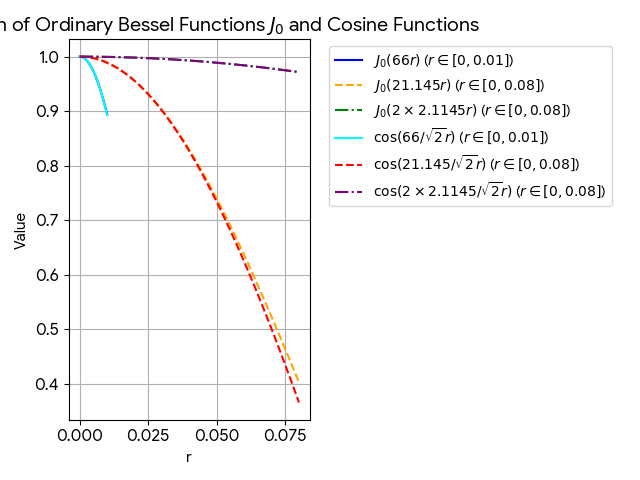
\includegraphics[width=0.75\textwidth]{curvature.png}
        \caption{Comparison of front position for Ta2O5 vs. SiO2 vs. C8H8, both the cylinder and the cartezian coordiante systems.}
        \label{fig:curvature}
    \end{figure}
    
    \item \textbf{The albedo formula:} 
    Shai came with the idea that our formula might not be right as it has been until now:
    \begin{equation}
        albedo = \frac{\sigma_{SB}T_s^4 - F/2}{\sigma_{SB}T_s^4 + F/2}
    \end{equation} 
    where $F$ is the flux between the wall and material. But, this formula does not zeroes the albedo for the vacuum case, while it should. 
    The short derivation: 
    \begin{equation}
        \sigma_{SB}T_D^4 = \sigma_{SB}T_s^4 + \frac{F}{2} 
    \end{equation}
    from marshak boundary condition. Another equality is:
    \begin{equation}
        \sigma_{SB}T_D^4 = \sigma_{SB}T_obs^4 + \frac{F}{2} 
    \end{equation}
    but watch that $T_{obs} = 0$ since no flux comes back from the vacuum, what means that: 
    \begin{equation}
        \sigma_{SB}T_D^4 = \frac{F}{2} 
    \end{equation}
    and so:
    \begin{equation}
        \sigma_{SB}T_s^4 = \sigma_{SB}T_D^4 - \frac{F}{2} = \frac{F}{2} - \frac{F}{2} = 0
    \end{equation}
    and so albedo is 0 in the vacuum case. 
    
    Watch that we have made an hidden assumption here that for the wall material $T_s = T_D$, which is not accurate. So we can agree that the incoming flux to the wall is $\sigma_{SB}T_D^4$ and the outgoing flux is $\sigma_{SB}T_D^4 - F$, since we have lost energy of $F\cdot dt$ from the material in the form of radiation in the time step. So the albedo calcuation should be like that:
    \begin{equation}
        albedo = \frac{\sigma_{SB}T_Foam^4 - F}{\sigma_{SB}T_Foam^4}
    \end{equation}
    where actually $T_{Foam}$ is the temperature of the wall material of the last foam cell before the interaction with the wall. Now according to how we loss energy when vacuum (which is $F = \sigma_{SB}T_D^4$) we have albedo 0 for vacuum.
    
\end{itemize}

\subsection{Decisions \& Conclusions}
\begin{itemize}
    \item \textbf{Ta$_2$O$_5$ curvature:} The current model for Ta$_2$O$_5$ is not accurate for Be and Vacuum, due to the fact that it assumes a small $\epsilon$, while in the reality $\epsilon = 1.28$. So we need a new model for it, or just accept the fact that the model is only valid for small $\epsilon$, meaning it won't work for Be and Vacuum when we have dense foam.
    \item \textbf{albedo formula:} The current formula for albedo is not accurate, and needs to be updated to the one we derived in the meeting. It should look like the following:
    \begin{equation}
        albedo = \frac{\sigma_{SB}T_{Foam}^4 - F}{\sigma_{SB}T_{Foam}^4}
    \end{equation}
\end{itemize}
%%%%%%%%%%%%%%%%%%%%%%%%%%%%%%%%%%%%%%%%%%%%%%%%
\newpage
\section{Meeting --- May 25, 2026}
\meetingmeta{May 25, 2026}{10:30 -- 12:30}{Shai, Yuval Kochavi}

\subsection{Agenda / Objectives}
\begin{itemize}
    \item Discuss the results of the model's curvature for Ta2O5.
    \item The legitimacy of lambda effective, using the simulation.
    \item Flux comparison between the simulation and the model, and even between the model and the experiments.
    \item Comparing the model front curvature to back's curvature (and maybe even other experiments) and see if we can get some insights from it.
\end{itemize}

\subsection{Discussion \& Key Progress}
\begin{itemize}
    \item \textbf{Ta$_2$O$_5$ curvature:} We kind of gave up on the idea of finding a new model for Ta$_2$O$_5$ curvature, and just accepted the fact that the current model is only valid for small $\epsilon$, meaning it won't work for Be and Vacuum when we have dense foam. We also discussed the fact that maybe we can find a new model for it, but it will be very hard to do so, and it might not be worth the effort. It's an experiment which involves a dense foam (tiny $\lambda_{R}$), with a big radius and a low-Z coating material (Be), which is a very extreme case, and maybe we can just accept the fact that our model is not accurate for it.
    \item \textbf{Legitimacy of lambda effective:} We discussed the validity of using an energy and front position for differnet radiuses, for nominal gold and a 100 times denser gold. We found that the we have a that for very tiny radiuses, the front position moves slower for both the nominal gold and the 100 times denser gold. We also found out that the ratio between the gold and foam energies is reasonable as the gold energy becomes closer to the foam's one. For a first look it looks like the lambda effective is legit, but the suspicison was that for small radiuses we have gotten that the 100 times denser gold has more energy than the gold in tiny radiuses, which means that it is not "dense to infinity" as we assumed. So, we moved to a 1 million times denser gold, and we found that the energy of the gold in tiny radiuses is smaller than the one in the 100 times denser gold, which means that it is really dense to infinity. No, we looked for the front location and found out that for the 1 million times denser gold, the front location is just like the 1D one, \textbf{what means that if the lambda effective is legit, it comes from the energy loss to walls at small radiuses, and not from wall collisions as we thoght.} So the next step is compare the energies for different radiuses in both simulation and model with ans without lambda effective, and if we see that the model with lambda effective is closer to the simulation, then we can say that the lambda effective is legit, and if not, we'll see. 
    \item \textbf{Flux comparison:} Shai came with the idea to compare the flux between the model and the simulation, and even between the model and the experiments. Since it's another great way to show the validation of the model. The way we can compute the flux of the model is by changing the cylender length (in back experiment it was at 0.5, 1 and 1.5 mm). Now, we can measure the flux at the edge from the time the front reaches the edge, and until the end (3 ns). So we will have to look at $T(l,t)$ and then compute the flux by $\sigma_{SB}T(l,t)^4$. Now when we will have to normalize the flux =, and compare to Back PRL, with the SiO2 low-energy. We can also compare the flux to the simulation, and see if we can get some insights from it.
    \item \textbf{Comparing the model front curvature to back's curvature:} We can compare the model front curvature to back's curvature. However, it might be hard, since in Back's experiment they have measured the flux curvature, and not the front curvature, so it won't be just putting the bessel function. We will need to take the temperature at the rellevant position, and then the flux, and thivk of the best way to compare it to the experiment. Shay gave me an article of Britian which might be helpful for it, since they took the prr and evolve it to find the flux.
\end{itemize}

\subsection{Decisions \& Conclusions}
\begin{itemize}
    \item \textbf{Ta$_2$O$_5$ curvature:} We will just accept the fact that our model is not accurate for Be and Vacuum when we have dense foam, and we won't try to find a new model for it, since it's an extreme case, and maybe it's not worth the effort.
    \item \textbf{Legitimacy of lambda effective:} We will compare the energies for different radiuses in both simulation and model with ans without lambda effective, and if we see that the model with lambda effective is closer to the simulation, then we can say that the lambda effective is legit, and if not, we'll see.
    \item \textbf{Flux comparison:} We will compute the flux of the model by changing the cylender length, and then measure the flux at the edge from the time the front reaches the edge, and until the end (3 ns). We will have to look at $T(l,t)$ and then compute the flux by $\sigma_{SB}T(l,t)^4$. 
    \item \textbf{Comparing the model front curvature to back's curvature:} We will compare the model front curvature to back's curvature, but we will need to take the temperature at the rellevant position, and then the flux.
\end{itemize}

%%%%%%%%%%%%%%%%%%%%%%%%%%%%%%%%%%%%%%%%%%%%%
\newpage
\section{Meeting --- May 26, 2026}
\meetingmeta{May 26, 2026}{15:10 -- 16:15}{Shai, Yuval Kochavi}

\subsection{Agenda / Objectives}
\begin{itemize}
    \item trying to see whether the lambda effective is legit.
\end{itemize}

\subsection{Discussion \& Key Progress}
\begin{itemize}
    \item 
\end{itemize}

\subsection{Decisions \& Conclusions}
We have came for 3 main conclusions without any decision.
\begin{itemize}
    \item $\lambda_{eff}$ doesn't really affect the energy that goes to the wall, but it does change the front location - a "1D" effect which we have proved not exsited in the simulation. 
    \item The best fit for the front location using \textbf{heyney is the one with $\lambda_{eff}$ and power of 2}, which also had a good fit for the energy. The best fit for the front location using \textbf{flattop is the ordinary gold loss or the one with $\lambda_{eff}$ and power of 10}, which also had a good fit for the energy. 
\end{itemize}

\end{document}
